% =================================================================================================
% File:			amm_utenti.tex
% Description:	Defiinisce la sezione relativa ad un capitolo del documento
% Created:		2015-04-21
% Author:		Tesser Paolo
% Email:		tesser.paolo@mashup-unipd.it
% =================================================================================================
% Modification History:
% Version		Modifier Date		Change											Author
% 0.0.1 		2015-04-21 			creato scheletro doc							Tesser Paolo
% =================================================================================================
%

% CONTENUTO DEL CAPITOLO
\section{Gestione degli utenti} % (fold)
\label{sec:gestione_utenti}
	

	\subsection{Contenuti Sezione} % (fold)
	\label{sub:contenuti_sezione}
		All'utente amministratore sono concessi permessi di gestione degli utenti.
		La gestione prevede le seguenti funzionalità:
		\begin{itemize}
			\item Visualizzazione dell'elenco di tutti utenti registrati sull'applicazione;
			\item Modifica permessi utente;
			\item Eliminazione profilo utente;
		\end{itemize}
		\begin{figure}[H]
			\centering
			\centerline{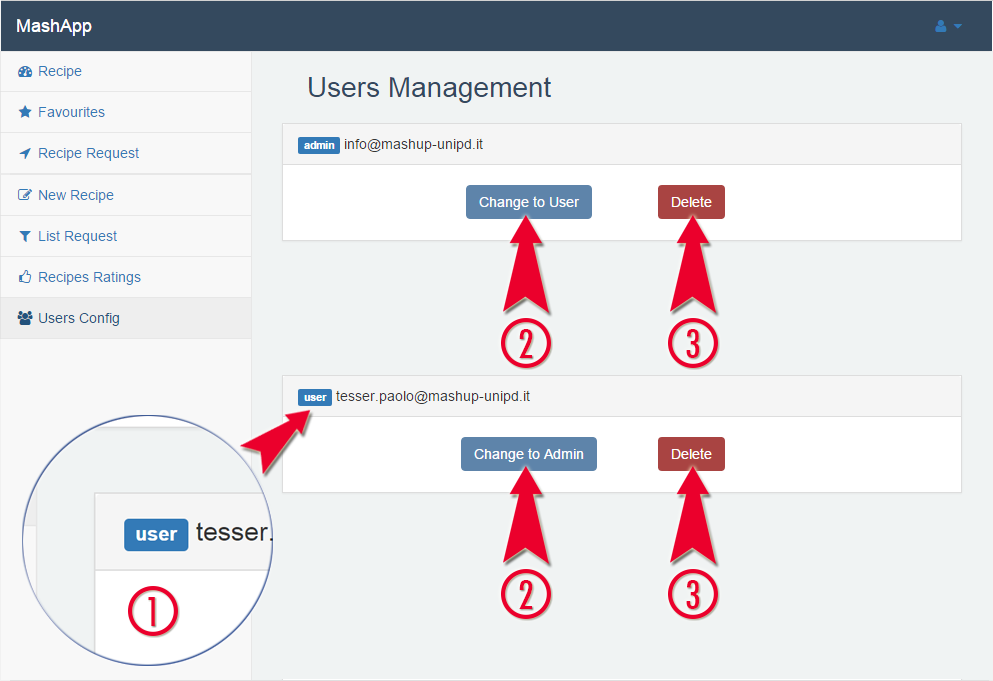
\includegraphics[width=14cm]{images/configurazione_utenti.png}}
			\caption{Gestione utenti}
			\label{fig:configurazione_utenti}
		\end{figure}
	% END

	\pagebreak
	\subsection{Visualizzazione elenco utenti}
		L'utente amministratore può visualizzare l'elenco (Figura: \ref{fig:configurazione_utenti}) di tutti gli utenti registrati nel sistema selezionando l'apposito pulsante dal Menu principale (Figura: \ref{fig:menu_principale_utente}) situato nella Home Page della dashboard\gloss{}.
		In questo elenco (Figura: \ref{fig:configurazione_utenti}) è possibile visualizzare tutti i dati di ciascun utente, modificare  i suoi permessi oppure eliminare un utente, purché esso non sia un amministratore a sua volta.
	% END	

	
	\subsection{Modifica permessi utente}
		L'utente amministratore può abilitare i permessi di amministratore ad un utente diverso da se stesso.\newline
		Per effettuare questa operazione è necessario accedere all'elenco degli utenti (Figura: \ref{fig:configurazione_utenti}) premendo l'apposito pulsante dal Menu principale di amministrazione (Figura: \ref{fig:menu_principale_utente}) dell'applicazione situato nella Home Page della dashboard (Figura: \ref{fig:screenshot}).
		La procedura prevede l'individuazione dell'utente nel sistema e la relativa pressione del pulsante \textbf{Change to admin}.\newline
		Una volta effettuata la selezione è richiesto di premere il pulsante di conferma dell'operazione per rendere effettive le modifiche.
	% END

	
	\subsection{Eliminazione utente}
		L'utente amministratore può eliminare un utente diverso da se stesso dal sistema.\newline
		Per effettuare questa operazione è necessario accedere all'elenco degli utenti (Figura: \ref{fig:configurazione_utenti}) premendo l'apposito pulsante dal Menu principale di amministrazione Figura: \ref{fig:menu_principale_utente}) dell'applicazione situato nella Home Page della dashboard (Figura: \ref{fig:screenshot}).
		La procedura prevede l'individuazione dell'utente nel sistema e la relativa pressione del pulsante \textbf{Delete}.\newline
		Una volta effettuata la selezione è richiesto di premere il pulsante di conferma dell'operazione di eliminazione per rendere effettive le modifiche.\newline
		ATTENZIONE: l'operazione di eliminazione utente non è reversibile.
	% END
		

% section Gestione degli utenti (end)